

\chapter{Data Set}
\section{Labelled Pupils in the Wild (LPW)}
\subsection{Description}

The data set "Labelled Pupils in the Wild" \cite{LPW} or short LPW was created by the Max Plank Institution and and contains 66 high-quality, high-speed eye region videos for the development and evaluation of pupil detection algorithms. All videos are labeled with the center of the pupil. 22 participant's eye region with five different ethnicities, five different eye colors were recorded.  

The goal of the data set was to record samples of participants under conditions that are present in the reality. By having strong reflections, wearing glasses, wearing make up and so on the data set becomes a difficult challenge for pupil detection algorithms and a good evaluation of the algorithms is possible.


\begin{figure}[ht]
    \centering
    \begin{subfigure}{.30\textwidth}
      \centering
      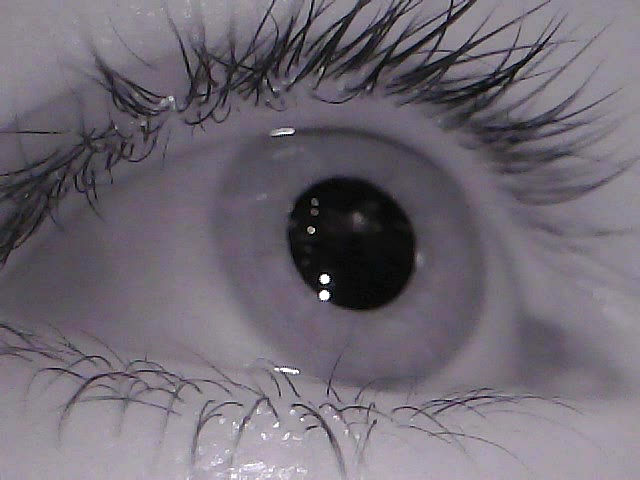
\includegraphics[width=.9\linewidth]{plots/eye_dataset/eye1.png}

      \label{fig:ds1}
    \end{subfigure}%
    \begin{subfigure}{.30\textwidth}
      \centering
      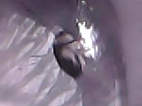
\includegraphics[width=.9\linewidth]{plots/eye_dataset/eye2.png}

      \label{fig:ds2}
    \end{subfigure}%
    \begin{subfigure}{.30\textwidth}
      \centering
      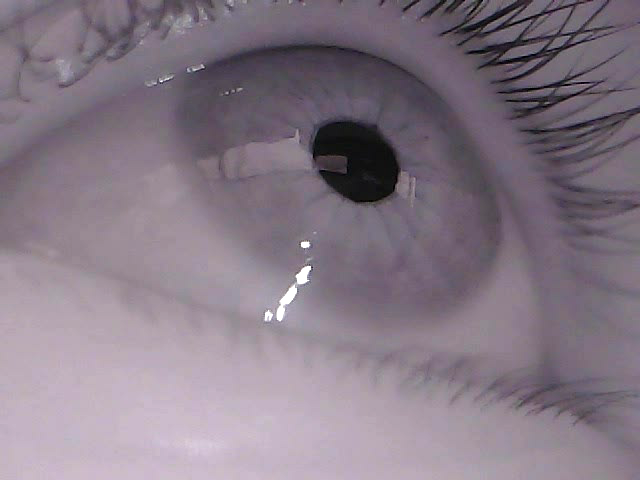
\includegraphics[width=.9\linewidth]{plots/eye_dataset/eye3.png}

      \label{fig:ds3}
    \end{subfigure}
    \caption{three example frames from the LPW data set.}
    \label{fig:example_frame}
    \end{figure}

    \subsection{Procedure}
    The participants were asked to look at a moving red ball as it moved around. The recording location was randomly picked and was in and around several buildings. Each location was chosen once, creating a diverse range of real life situations. 

    For the recording a high-speed Pupil Pro head-mounted eye tracker was used that took 95 frames per second with a resolution of 640x480 pixels. With this frame rate even fast eye movements last through several frames making it more robust to detect the pupil.


    \begin{table}[h]
      \centering 
      \begin{minipage}{0.7\textwidth}
        \centering
        \begin{tabular}{|c|c|}
          \hline
          Location & Number of Videos \\
          \hline
          Outside & 34.3\% \\
          Inside & 65.7\% \\
          \hline
        \end{tabular}
        \caption{Location of recordings}
        \label{tab:location}
      \end{minipage}\hfill
      \begin{minipage}{0.7\textwidth}
        \centering
        \begin{tabular}{|c|c|}
          \hline
          Light source & Percentage of recordings \\
          \hline
          Natural light & 84.7\% \\
          Artificial light & 33.6\% \\
          \hline
        \end{tabular}
        \caption{Light Source of recordings}
        \label{tab:light_source}
      \end{minipage}
    \end{table}

    \subsection{Ground truth annotation}
    In many cases the pupil area has a clear boundary the center can be annotated easily. One or two points inside the pupil were manualy selected and used as seed points. From these point area with the same intensity value are extracted and used for annotation.  But in some difficult scenarios this method was not possibl because of strong noise over the pupil. In this case the additional information gained from the participants following a red fall with their eyes was used to create the labels. The frames then were manually annotated and this data was then used as calibration data to cross reference the center of the pupil with the position of the red ball. 
    
    The complete data set has labels for the center of the pupil for every frame.
    Given the ground truth annotation, it is possible to evaluate algorithms and compare them to each other.
    \subsection{Folder structure}
    The folder stands for the part, file number stands the participants and the file extension for the file type. The text file contains the ground truth annotation of the pupil center in x and y coordinates for each frame.
    
    The labels.ods file contains the information about the location, light source, vision aid used, prescription, nationality, eye color and gender. The README.txt file contains the information about the data set and the folder structure.
    
    The folder structure is shown in the following tree diagram.

    \dirtree{%
    .1 LPW/.
.2 labels.ods.
.2 README.txt.
.2 1.
.3 1.avi.
.3 1.txt.
.3 4.avi.
.3 4.txt.
.3 ....
.2 2.
.3 4.avi.
.3 4.txt.
.3 ....
.2 ....
.3 ....
.2 22. 
.3 ....
}
    \section{Eye characteristics}
    \subsection{Anatomy of the eye}
    The eye is surrounded by the \textbf{eye lid}. Its purpose is to shield the eye from debris and lubricate the eye by spreading tears over its surface with each blink. Then there are four different parts of the eye that matters for pupil detection. The white part of the eye is the \textbf{sclera} and is separated from the \textbf{iris} by the \textbf{limbus}.
    \begin{table}[h]
      \centering 
      \begin{minipage}{0.7\textwidth}
        \centering
        \begin{tabular}{|c|c|c|}
          \hline
          Name & Radius & Additional Information \\
          \hline
          Iris & 12 mm & in average\\
          Pupil & 2-9 mm & varies with light intensity\\
          \hline
        \end{tabular}
        \caption{Oversight iris and pupil radius}
        \label{tab:eye_char}
      \end{minipage}\hfill
    \end{table}
 

    The iris regulates the radius size of the \textbf{pupil} is and thereby regulates how much light comes through the pupil. The pupil is in the center of the iris and is the black part of the eye. The Darker the environment is, the larger the pupil radius. The Iris is colored and can be blue, green/hazle, brown, gray, amber and black. There are also other colors but they are in connection with health issues or genetic defects and play no role in this thesis. 

    The most important fact for pupil detection is that the iris, pupil and sclera have different brightness values. The pupil is the darkest area in the eye, the sclera is the brightest and the iris is in between. Depending on the color of the iris, the brightness value can vary.  Those characteristics are often used in pupil detection algorithms and will be discussed in the next chapter.
    \begin{figure}[ht]
      \centering
      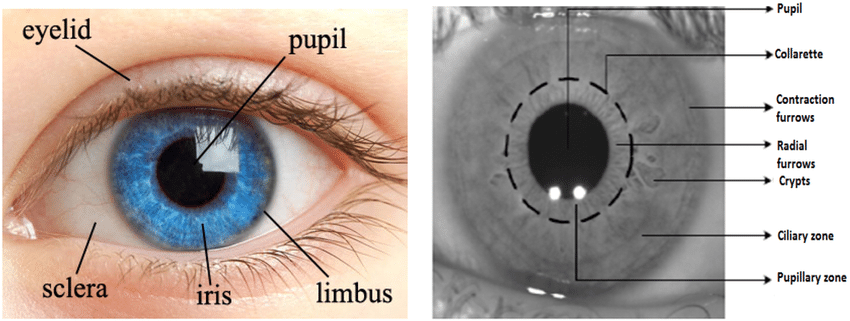
\includegraphics[width=0.98\textwidth]{plots/eye_dataset/Various-characteristics-of-an-eye-and-its-iris-texture-7.png}
      \caption{Overview of the different parts of the eye.}
      \label{fig:eye_anatomy}
    \end{figure}
    There can also be reflections of the environment be seen in the eye. This reflection is called \textbf{purkinje reflection} and can temper with pupil detection algorithms accuracy and therefore is a challenge for pupil detection algorithms.


    \subsection{Image characteristics}
    \subsubsection{Histogram}
    When inspecting the histogram of a randomly chosen frame from the LPW data set, it can be seen that the histogram shows different peaks in different intensities. In this particular example it can be seen that the peak between 0 and 50 corresponds to the pupil it self. This can be be seen in figure \ref{fig:hist1} because when comparing both histograms the lowest peak stays unchanged. The intensity of the iris is therefore between 90 and 150.

    \begin{figure}[ht]
      \centering
      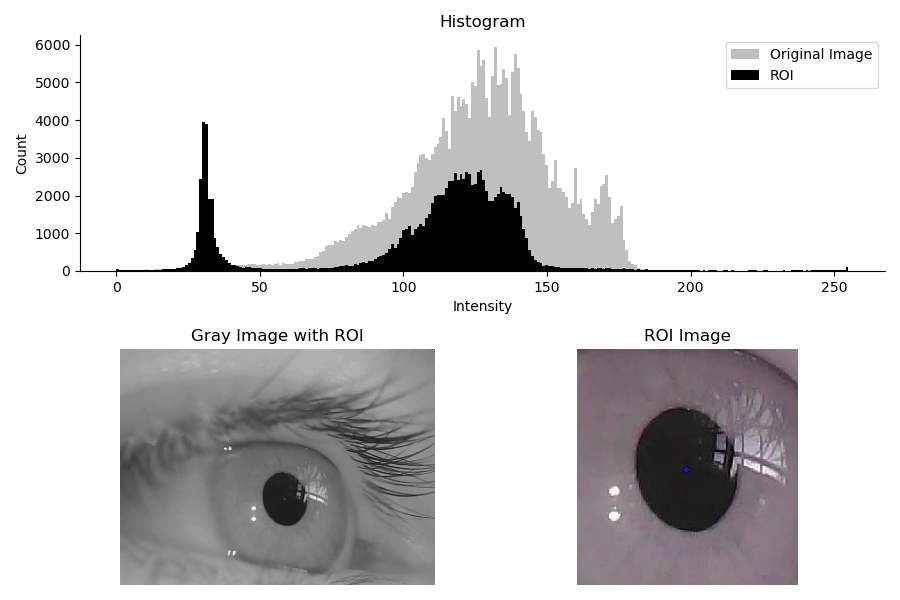
\includegraphics[width=0.9\textwidth]{plots/histogram_with_roi.png}
      \caption{Comparison histogram of the whole image and the region of interest.}
      \label{fig:hist1}
    \end{figure}

    The sclera is the brightest part of the eye but in this frame the skin intensity will be around the same magnitude as the sclera intensity. Subtracting the ROI from the original picture will result in a histogram almost only containing the skin and sclera. The histogram is therefore a strong tool for eye segmentation. 

    If there is more reflection on the pupil, the histogram will also change in its shape. The peak created by the pupil will shrink and flatten out. The mean of the histogram will increase as dark points are substituted by brighter points. This ultimately makes it hard for using a fixed threshold for segmentation. Using Histogram equalization increases the contrast of the image but stretches the peak into a wider intensity range. 

    Also interesting to inspect is one pixel row of the image with their intensity values. Here it can be observed that the pupil creates a valley in the intensity values. The reflection on the pupil generates a peak right after the valley. This can be seen in figure \ref{fig:row_intens}.
    \begin{figure}[ht]
      \centering
      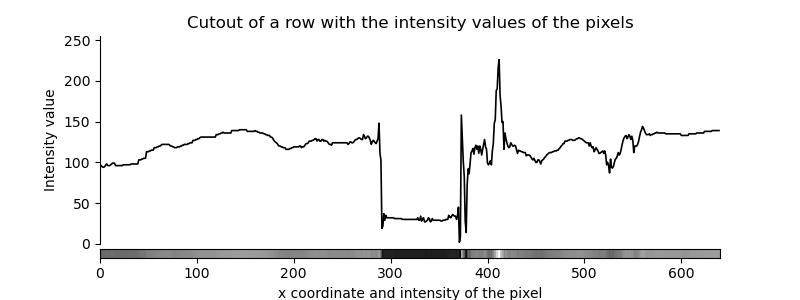
\includegraphics[width=0.9\textwidth]{plots/row_intensity_valles.png}
      \caption{Plot of the intensity values of one pixel row.}
      \label{fig:row_intens}
    \end{figure}

    The x coordinate represents the pixel at this coordination and the y coordinate represents the intensity value of the pixel. 

    The conclusion is, that the histogram is a strong tool to gain insight information of the frame but can vary a lot depending on the environment, therefore adaptive algorithms have to be used. 
    

   
    \subsubsection{Gradients}
    As already shown in the previous subsection, the pupil creates a valley in the intensity values. This is also reflected in the gradient of the image. The gradient responds strongly to the change of intensity in the transition from the pupil to the iris. The orientation of the gradient points from the pupil towards the iris and can be of great help for edge detection. The gradient is calculated by using the Sobel operator. The Sobel operator is a discrete differentiation operator. It convolves the image with a differential kernel and therefore emphasizes regions with high spatial frequency. The Sobel operator will be discussed in a later chapter in more detail. But for know it's important to get an overview of the different characteristics of the eye.

    

    \begin{figure}[ht]
      \centering
      % First row: 3 images
      \begin{subfigure}{.33\textwidth}
        \centering
        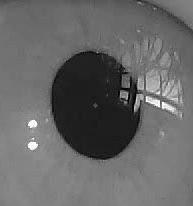
\includegraphics[width=.9\linewidth]{plots/eye_dataset/roi.png}
        \caption{Image of ROI}
        \label{fig:roig}
      \end{subfigure}%
      \begin{subfigure}{.33\textwidth}
        \centering
        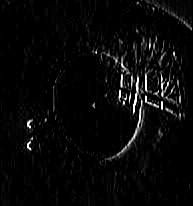
\includegraphics[width=.9\linewidth]{plots/eye_dataset/sx.png}
        \caption{Gradient in x\textbf{$G_{x}$}}
        \label{fig:sx}
      \end{subfigure}%
      \begin{subfigure}{.33\textwidth}
        \centering
        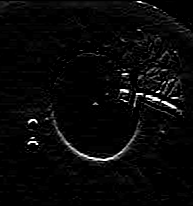
\includegraphics[width=.9\linewidth]{plots/eye_dataset/sy.png}
        \caption{Gradient in y \textbf{$G_{y}$}}
        \label{fig:sy}
      \end{subfigure}
      % Second row: 2 images
      \begin{subfigure}{.33\textwidth}
        \centering
        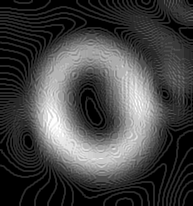
\includegraphics[width=.9\linewidth]{plots/eye_dataset/mag.png}
        \caption{Magnitude \textbf{$G$}}
        \label{fig:mag}
      \end{subfigure}%
      \begin{subfigure}{.33\textwidth}
        \centering
        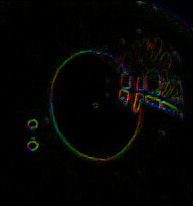
\includegraphics[width=.9\linewidth]{plots/eye_dataset/direction.png}
        \caption{Orientation \textbf{$\theta$}}
        \label{fig:orientation}
      \end{subfigure}
      \caption{Plot of gradient characteristics of the ROI.}
      \label{fig:gradient}
      \end{figure}
      
      The gradient in x direction is shown in figure \ref{fig:sx} and the gradient in y direction is shown in figure \ref{fig:sy}. The magnitude of the gradient is shown in figure \ref{fig:mag} and the orientation of the gradient is shown in figure \ref{fig:orientation}. Depending on the environment, the gradient itself could already sufficient for pupil detection. In image processing the gradient is often used for edge detection and all sorts of different filters. Used correctly it can be very powerful. The magnitude is calulated by the following formula: 

      \begin{equation}
        \label{eq:magnitude}
        \begin{split}
          G = \sqrt{G_x^2 + G_y^2}
        \end{split}
      \end{equation}
      Because we have the gradient in x and y direction, we can calculate the orientation of the magnitude by using the following formula: 
      \begin{equation}
        \label{eq:orientation}
        \begin{split}
          \theta  = \arctan{\frac{G_y}{G_x}}
        \end{split}
      \end{equation}
      The orientation is calculated in radians and can be converted to degrees by multiplying it with $\frac{180}{\pi}$. The orientation is perpenticular to the edge and points in the direction of the gradient. Because the pupil is darker than the iris, the gradient points from the pupil to the iris. 

    \subsubsection{Noise}
      In the data set there are different kind of noise. The most common noise is the noise created by the camera. This noise is called \textbf{Gaussian noise}. Gaussian noise is a statistical noise having a probability density function equal to that of the normal distribution, which is also known as the Gaussian distribution. The noise is created by the camera and is therefore not dependent on the environment. The noise is therefore not a problem for the pupil detection algorithm.

      Considering that the goal is to detect the pupil there can also be other noise that can be problematic. \textbf{Reflection} of the environment can have an impact on the accuracy of the algorithm and destroy information about the pupil. Also the \textbf{eyelashes} can be problematic. They are very dark and therefore temper with the edges of the pupil and iris. Especially when the eyelashes are in front of the pupil. Also if make up is used. 

      Another Noise term can be that the eye is not constantly open. The \textbf{eyelid} can cover parts of the pupil or even the whole pupil. Then also glasses or lenses can add noise to the image. 